% This file was created by tikzplotlib v0.9.8.
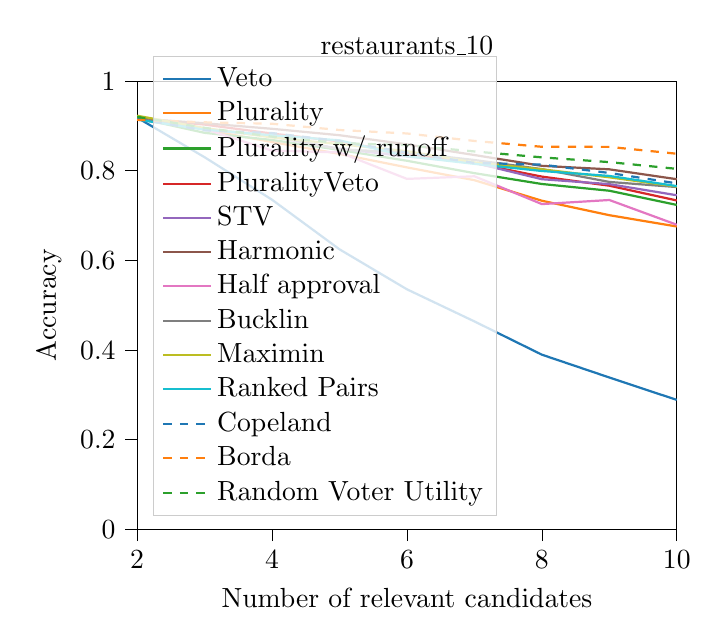
\begin{tikzpicture}

\definecolor{color0}{rgb}{0.12156862745098,0.466666666666667,0.705882352941177}
\definecolor{color1}{rgb}{1,0.498039215686275,0.0549019607843137}
\definecolor{color2}{rgb}{0.172549019607843,0.627450980392157,0.172549019607843}
\definecolor{color3}{rgb}{0.83921568627451,0.152941176470588,0.156862745098039}
\definecolor{color4}{rgb}{0.580392156862745,0.403921568627451,0.741176470588235}
\definecolor{color5}{rgb}{0.549019607843137,0.337254901960784,0.294117647058824}
\definecolor{color6}{rgb}{0.890196078431372,0.466666666666667,0.76078431372549}
\definecolor{color7}{rgb}{0.737254901960784,0.741176470588235,0.133333333333333}
\definecolor{color8}{rgb}{0.0901960784313725,0.745098039215686,0.811764705882353}

\begin{axis}[
legend cell align={left},
legend style={
  fill opacity=0.8,
  draw opacity=1,
  text opacity=1,
  at={(0.03,0.03)},
  anchor=south west,
  draw=white!80!black
},
tick align=outside,
tick pos=left,
title={restaurants\_10},
x grid style={white!69.0196078431373!black},
xlabel={Number of relevant candidates},
xmin=2, xmax=10,
xtick style={color=black},
y grid style={white!69.0196078431373!black},
ylabel={Accuracy},
ymin=0, ymax=1,
ytick style={color=black}
]
\addplot [thick, color0]
table {%
2 0.9186
3 0.8302
4 0.7354
5 0.6248
6 0.5356
7 0.464
8 0.3898
9 0.3389
10 0.2889
};
\addlegendentry{Veto}
\addplot [thick, color1]
table {%
2 0.9204
3 0.8919
4 0.8641
5 0.8377
6 0.8075
7 0.779
8 0.7332
9 0.7009
10 0.6757
};
\addlegendentry{Plurality}
\addplot [thick, color2]
table {%
2 0.918
3 0.8846
4 0.8687
5 0.8465
6 0.8223
7 0.7947
8 0.7705
9 0.7555
10 0.7238
};
\addlegendentry{Plurality w/ runoff}
\addplot [thick, color3]
table {%
2 0.9165
3 0.903
4 0.883
5 0.8655
6 0.8378
7 0.8169
8 0.787
9 0.7667
10 0.7338
};
\addlegendentry{PluralityVeto}
\addplot [thick, color4]
table {%
2 0.915
3 0.8935
4 0.8759
5 0.8493
6 0.8319
7 0.8177
8 0.7812
9 0.7702
10 0.7454
};
\addlegendentry{STV}
\addplot [thick, color5]
table {%
2 0.9168
3 0.906
4 0.8936
5 0.8793
6 0.8589
7 0.8351
8 0.811
9 0.8032
10 0.7812
};
\addlegendentry{Harmonic}
\addplot [thick, color6]
table {%
2 0.9158
3 0.8934
4 0.845
5 0.841
6 0.7819
7 0.7877
8 0.7257
9 0.7348
10 0.6796
};
\addlegendentry{Half approval}
\addplot [thick, white!49.8039215686275!black]
table {%
2 0.916
3 0.8934
4 0.8784
5 0.8478
6 0.8408
7 0.824
8 0.8037
9 0.7751
10 0.7637
};
\addlegendentry{Bucklin}
\addplot [thick, color7]
table {%
2 0.9228
3 0.8954
4 0.8743
5 0.8594
6 0.8438
7 0.8186
8 0.8033
9 0.7854
10 0.7647
};
\addlegendentry{Maximin}
\addplot [thick, color8]
table {%
2 0.9142
3 0.8917
4 0.8792
5 0.8679
6 0.8325
7 0.8154
8 0.7995
9 0.7885
10 0.7658
};
\addlegendentry{Ranked Pairs}
\addplot [thick, color0, dashed]
table {%
2 0.9156
3 0.8901
4 0.8841
5 0.8663
6 0.8407
7 0.8175
8 0.8137
9 0.7951
10 0.7719
};
\addlegendentry{Copeland}
\addplot [thick, color1, dashed]
table {%
2 0.9136
3 0.9081
4 0.9049
5 0.8909
6 0.8832
7 0.8665
8 0.8535
9 0.8533
10 0.838
};
\addlegendentry{Borda}
\addplot [thick, color2, dashed]
table {%
2 0.9204
3 0.8958
4 0.8761
5 0.8617
6 0.8571
7 0.8431
8 0.8299
9 0.8193
10 0.8043
};
\addlegendentry{Random Voter Utility}
\end{axis}

\end{tikzpicture}
